%
% path-finding
% @author Tobias Weber <tweber@ill.fr>
% @date 2021
% @license see 'LICENSE' file
%

\chapter{Path-finding Details and Implementation}
\label{ch:impl}

In this chapter we describe the individual steps of the strategy (see p. \pageref{sec:strategy}) in detail
and present an implementation in C++ \cite{Stroustrup2008, Stroustrup2018}. Specifically,
the latest version 20 of the C++ standard \cite{ISOCPP20} was employed in the creation of the software
together with the Boost C++ template libraries \cite{web_boost}. The source code for the implementation
can be found in the directory \lstinline|./src/core| together with the library routines in \lstinline|./src/libs|
of the repository at \url{https://code.ill.fr/scientific-software/takin/paths}. Stable versions of the
source code have furthermore been registered under the DOI \href{https://doi.org/10.5281/zenodo.4625649}{10.5281/zenodo.4625649}.

Section \ref{sec:tasmodel} is dedicated to modelling the triple-axis spectrometer (TAS), 
section \ref{sec:buildpath} discusses the steps involved in building up the instrument path, 
and section \ref{sec:exepath} focuses on executing the instrument motion along the path.
The graphical user interface is presented separately, namely in chapter \ref{ch:gui}.





% -----------------------------------------------------------------------------
% instrument model
% -----------------------------------------------------------------------------
\section{TAS instrument modelling}
\label{sec:tasmodel}

The instrument space comprising the triple-axis spectrometer, the walls and obstacles as well as the floor is modelled in
the class \lstinline[language=C++]|InstrumentSpace|. It also serves as high-level interface for loading and saving
the instrument geometry and states, signalling mechanisms for state changes using the publish-subscribe mechanism
via Boost.Signals2 \cite{web_boost_signals}, as well as checking the instrument for collisions.

The classes \lstinline[language=C++]|Instrument| and \lstinline[language=C++]|Axis| contain the actual instrument definition.
The spectrometer is modelled as a hierarchy of the three principal axes, namely monochromator, sample and analyser.
Each axis has three local coordinate systems, namely the rotation relative to the incoming and outgoing vector, respectively,
and an internal rotation which is decoupled from the other local rotations.
Geometrical objects are derived from the abstract, purely virtual class \lstinline[language=C++]|Geometry| and can be
coupled to any of these three local coordinate systems.
This makes it possible to model neutron-optical components attached to the either the incoming or outgoing path of the
neutron beam at the specific axis. It furthermore makes it possible to have components which rotate independently of
the axis.
Physically, the outgoing coordinate system is equal to the scattering angle, while the internal angle corresponds
to the crystal rocking angle (see Ch. \ref{ch:xtal}).
The transformation matrices corresponding to the three local coordinate systems are calculated as follows:

\begin{equation}
\begin{split}
	T_{\mathrm{in}}^{i} & \ =\  T_{\mathrm{out}}^{i-1} \cdot P^{i} \cdot R\left(\theta_{\mathrm{in}}^{i}\right), \\
	T_{\mathrm{int}}^{i} & \ =\  T_{\mathrm{in}}^{i} \cdot R\left(\theta_{\mathrm{int}}^{i}\right), \\
	T_{\mathrm{out}}^{i} & \ =\  T_{\mathrm{in}}^{i} \cdot R\left(\theta_{\mathrm{out}}^{i}\right).
\end{split}
\end{equation}

Here, $T_{\mathrm{in,\, int,\, out}}^{i}$ names the transformation matrices of the incoming, internal (decoupled) and outgoing
coordinate system of axis $i$, respectively.
$T_{out}^{i-1}$ is the outgoing transformation of the preceding instrument axis, or the identity if it is the first axis in the hierarchy.
$R\left(\theta_{\mathrm{in,\, int,\, out}}\right)$ are the corresponding rotation matrices and $P^i$ is the translation
of the local coordinate origin of the respective axis $i$.
The situation is depicted in Fig. \ref{fig:tas_axes}.


\begin{figure*}
	\begin{minipage}{0.45 \textwidth}
		\begin{center}
			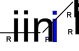
\includegraphics[width = 0.75 \textwidth]{figures/axis}
		\end{center}
	\end{minipage}
	%\hspace{1cm}
	\begin{minipage}{0.45 \textwidth}
		\begin{center}
			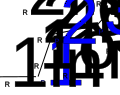
\includegraphics[width = 0.95 \textwidth]{figures/axes}
		\end{center}
	\end{minipage}
	\caption{Left panel: Local transformations for an axis. The symbols $R_{\mathrm{x}}^i$ are shorthands
	for the rotation matrices $R\left( \theta_{\mathrm{x}}^i \right)$, with $x = \left\{ \mathrm{in,\, int,\, out} \right\}$.
	$P^i$ is the point of origin for the axis.
	Right panel: Three coupled axes build up the triple-axis spectrometer, with axes 1, 2, and 3 naming the monochromator,
	the sample, and the analyser axis, respectively.
	\label{fig:tas_axes}}
\end{figure*}

% -----------------------------------------------------------------------------





% -----------------------------------------------------------------------------
% path building
% -----------------------------------------------------------------------------
\section{Path-building}
\label{sec:buildpath}

As discussed in chapter \ref{sec:tasrobot}, path-creation will be based on the angular configuration space
(as opposed to -- for example -- crystal configuration space). The top-level C++ class for creating the path
is named \lstinline[language=C++]|PathBuilder|. It mainly calls the low-level routines from the geometry
library situated in the directory \lstinline|./src/libs| of the source code repository.


\subsection{Angular configuration space}
As the obstacles do not have any geometrically primitive shape in angular configuration space, we iterate
through the configuration space on a two-dimensional grid and create a bitmap of allowed and forbidden
positions. The grid extends towards the scattering angles $2\theta_S \in \left[ -180^{\circ},\, 180^{\circ} \right]$ and monochromator angles of $2\theta_M \in \left[0^{\circ},\, 180^{\circ} \right]$, where, for the monochromator, we do
not the full angular range as this is not possible in real instruments which has the monochromator at a fixed position
and only scatters in one direction. The sample scattering angle, on the other hand, needs the full angular range as
scattering on both sides of the axis is done in practice.

To check for the allowed positions, the instrument model as described in sec \ref{sec:tasmodel} is moved to
each $\left( 2\theta_S,\, 2\theta_M \right)$ position on the grid and tested for collisions with the walls or with
itself. Even though the instrument model itself is a three-dimensional representation of the spectrometer, we
can nevertheless simplify the collision detection checks to a two-dimensional plane. The reason for this is
that all possible obstacles in the instrument path, for instance walls and pillars, are upright and do not have
any sloped angles. The same is true for the instrument itself.

Collision calculation on the two-dimensional grid is spread out on several processor cores using 
the \lstinline[language=C++]|thread_pool| \cite{web_boost_asio_threadpool} class from the 
Boost.Asio \cite{web_boost_asio} asynchronous input/output library.


\subsection{Contour tracing}


\subsection{Line-segment generation and simplification}


\subsection{Generation of convex regions}


\subsection{Calculation of the Voronoi diagram}
\label{sec:voronoi}


\subsection{Simplification of the Voronoi diagram}


% -----------------------------------------------------------------------------





% -----------------------------------------------------------------------------
% instrument motion
% -----------------------------------------------------------------------------
\section{Instrument movement}
\label{sec:exepath}


\subsection{Determination of the start and end coordinates}



\subsection{Calculation of Dijkstra's shortest path}
\label{sec:dijkstra}


% -----------------------------------------------------------------------------
